\laborator{Основы программирования в пакете Mathcad}

\goal ознакомиться с возможностями языка программирования математического пакета Mathcad; рассмотреть основные операторы и приемы программирования в Mathcad.

\subsubsection{Теория}
Язык программирования Mathcad содержит все элементы языка высокого уровня, необходимые для математических расчетов. Кроме того, он содержит дополнительно сотни встроенных функций и операторов системы Mathcad, имеет возможности численного и символьного расчета различных величин, и поэтому по эффективности не уступает профессиональным системам программирования.

Все операторы и элементы языка программирования Mathcad расположены на рабочей панели \menu[,]{Математика, Программирование}. 
Чтобы написать программу, прежде всего для нее должен быть создан специальный обособленный от остального документа блок. Выглядит он как две черных вертикальных линии с маркерами, в которые заносятся те или иные выражения алгоритма. Чтобы построить единичный элемент программного блока, нажмите панели кнопку "Программа" (клавишей \keys{]}). При этом в области курсора появится следующий объект:
\begin{center}
	
\includegraphics{new-prog-1.png}
\end{center}

Обычно программа содержит больше чем две строки, поэтому лучше сразу задать блок из 5-6 маркеров. Сделать это можно использовать клавишу \keys{\enter}.

Программный блок можно создать и внутри уже заданного блока. Для этого используйте один из стандартных способов, поставив курсор в маркер любого из операторов программирования:
\begin{center}
	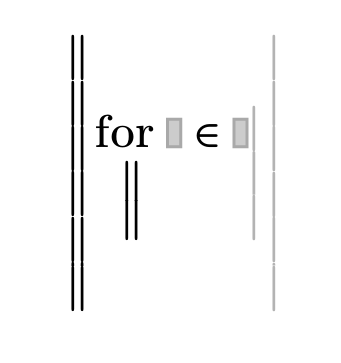
\includegraphics{new-prog-2.png}
\end{center}

Созданный таким образом блок выглядит как параллельная главному блоку линия. Выражения, внесенные в него, будут обособлены от остальной программы, и выполнение соответствующих действий будет связано только с оператором, к которому относится внутренний блок.
Для присвоения значений переменным и функциям в программах Mathcad используется специальный оператор: «$\leftarrow$» --- «Локальное определение» (панель «Программирование») или сочетание \keys{\shift + [} . Использовать оператор обычного присваивания «:=» в программах нельзя.

Присваивание значений в программах имеет ряд особенностей. Присвоение величин используемым алгоритмом функциям и переменным может быть произведено как в самой программе, так и выше нее. Если значение переменной или функции присваивается в программе посредством оператора «$\leftarrow$», то такая переменная или функция будет являться локальной, то есть она будет видимой только в рамках программы. Как-то повлиять на объекты вне программы она не сможет (равно как извне к ней нельзя будет получить доступ). Если переменная или функция задаются выше программы с помощью оператора «:=», то она будет обладать глобальной видимостью, то есть такая переменная или функция будет доступна любому нижележащему объекту, в том числе и коду программ. Однако программа может только прочитать значение глобальной переменной или вызвать глобальную функцию. Как-то изменить значение глобальной переменной или функции программа не может. Если программа должна осуществлять какую-то модификацию объекта (например, возводить все элементы массива в квадрат), то результат своей работы она должна возвращать.

Локальные переменные и функции имеют приоритет над глобальными в рамках «родной» программы. Это означает, что если имеется локальная и глобальная переменные (или функции) с одним именем, то обращение по этому имени будет адресоваться к локальной переменной (или функции).

\primer{Задайте переменную \mc{А}, далее создайте программный блок, где этой же переменной присвойте новое значение и выведите его на печать. После выполнения блока распечатайте значение переменной. Значение переменной, полученной в результате выполнения программы, присвойте новой переменной, что бы она была доступна вне программы. }

\begin{center}
	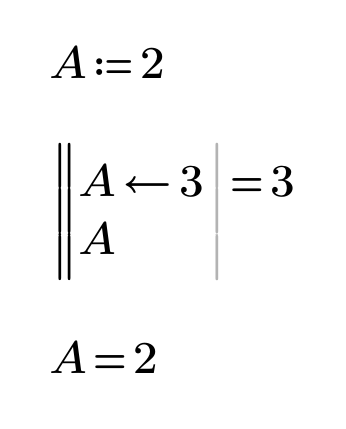
\includegraphics{new-prog-3.png}
\end{center}

\primer{Значение переменной, полученной в результате выполнения предыдущей программы, присвойте новой переменной, чтобы она была доступна вне программы. }

\begin{center}
	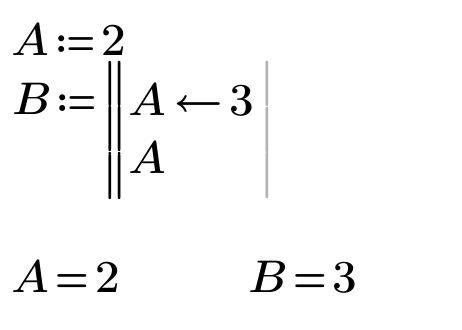
\includegraphics{new-prog-4.png}
\end{center}

Как видно из задания, в результате выполнения программы значение переменной \mc{А} изменено не было.

Mathcad позволяет в теле программы задать локальную пользовательскую функцию. Создаются локальные функции точно так же, как обычные (только в качестве оператора присваивания используется ). Вызвать локальную функцию можно только из нижележащих строк программы. Вне программы она не доступна.

\primer{Задайте пользовательскую функцию $f(x,y,z) = sin(x)+sin(y)+sin(z)$. Обратитесь в теле программы к данной функции несколько раз и распечатайте полученное значение.}
\begin{center}
	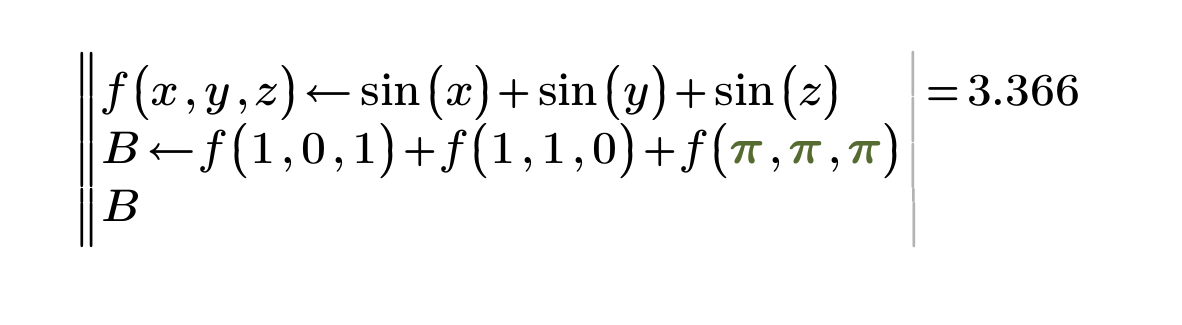
\includegraphics{new-prog-5.png}
\end{center}

Построение программ проводится с использованием специальных управляющих операторов, вроде оператора цикла \mc{for} или оператора условия \mc{if}. Чтобы задать нужный оператор, используйте соответствующие кнопки панели \menu[,]{Математика, Программирование}. Просто набрать оператор с клавиатуры нельзя – он будет воспринят системой Mathcad как неизвестная функция.

Такие операторы, как \mc{if}, \mc{for}, \mc{while}, активируют код, помещенный в их левый маркер, в том случае, если выполняется условие в правом. Для задания условия используются операторы булевой алгебры <<$=$>>, <<$>$>>, <<$<$>> и т.д. Можно задать и комплекс условий, задействовав оператор логического И <<$\land$>> панели «Булева алгебра», или оператор логического ИЛИ <<$\lor$>> .

\subsection*{Операторы цикла (\mc{for}, \mc{while})}

Оператор простого цикла \mc{for} позволяет организовать выполнение операции или проверку условия для ряда конкретных значений переменной. Оператор for задается с помощью команды панели «Программирование» или сочетанием клавиш \keys{\ctrl + \shift + '}. Оператор \mc{for} имеет три маркера:
\begin{center}
	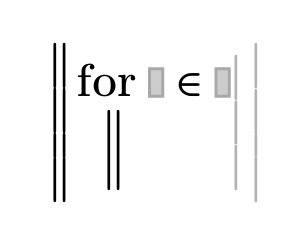
\includegraphics{new-prog-6.png}
\end{center}


В двух верхних маркерах, соединенных символом принадлежности, задается имя переменной, по которой организуется цикл, и ряд принимаемых ею значений. В нижнем маркере определяется операция или комплекс операций, которые должны быть выполнены для каждого значения переменной. Ряд значений переменной обычно представляет собой последовательность целых чисел, которая задается с помощью ранжированной переменной. Для этого в правый верхний маркер вводится оператор ранжированной переменной (панель «Матрица»), по умолчанию ряд будет содержать целые значения с шагом 1. Если значения переменной должны изменяться с меньшим или большим шагом, то это можно сделать, введя в правом маркере оператора ранжированной переменной через запятую первое и второе значения в ряде переменной (разница между ними и задаст шаг).
\begin{center}
	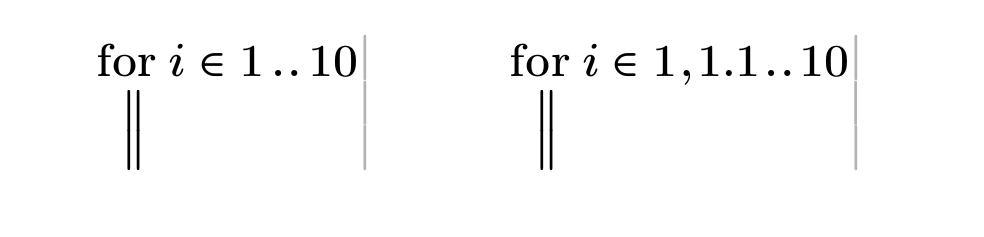
\includegraphics{new-prog-7.png}
\end{center}


Если операция или комплекс операций должны быть просчитаны при ряде некоторых конкретных значений переменной, причем ряд этот нельзя задать математически в общем виде, его можно непосредственно определить в правом верхнем маркере оператора \mc{for} в виде вектора:
\begin{center}
	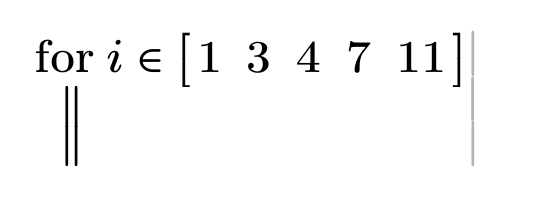
\includegraphics{new-prog-8.png}
\end{center}

С помощью второго оператора цикла \mc{while} (Пока) (сочетание клавиш \keys{\ctrl+]} ) можно организовать цикл, который будет работать до тех пор, пока выполняется некоторое условие. Оператор \mc{while} имеет два маркера, в которые вводятся соответственно условие работы цикла и выражения операций, которые должны быть проделаны на каждом его витке:
\begin{center}
	
\includegraphics{new-prog-9.png}
\end{center}


В цикле \mc{while} количество его витков не нужно определять явно. Итерации будут совершаться до тех пор, пока будет выполняться условие в правом маркере.

\begin{center}
	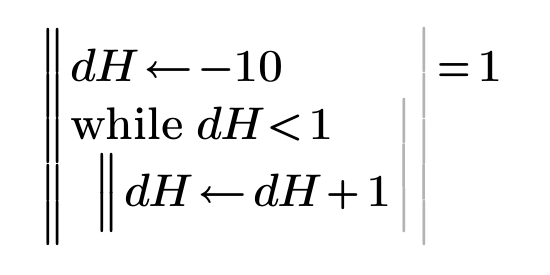
\includegraphics{new-prog-10.png}
\end{center}

Если возникает необходимость прервать работу цикла, то можно использовать оператор \mc{break} (Прервать). Ввиду того, что цикл бывает нужно остановить при выполнении некоторого условия, оператор \mc{break} почти всегда используется с условным оператором \mc{if}.

\primer{Используя операторы цикла, замените значения элементов произвольного массива A размерностью 3х3 их квадратами. Полученные значения присвойте новой переменной.}
\begin{center}
	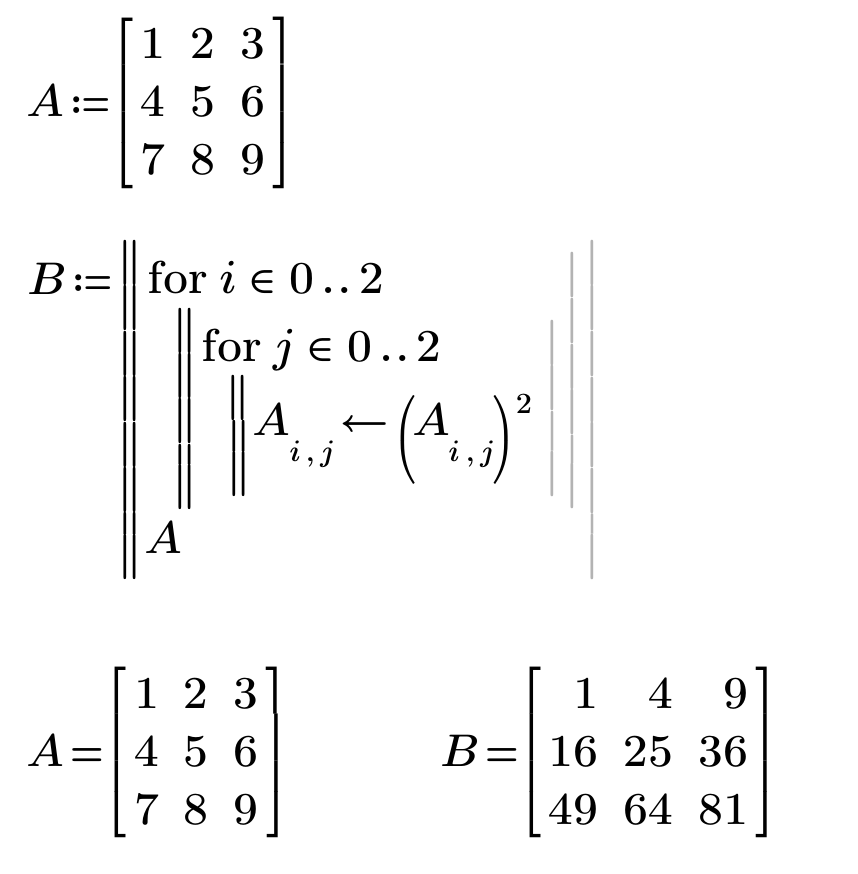
\includegraphics{new-prog-11.png}
\end{center}


\subsection*{Условные операторы (\mc{if}, \mc{else})}
Условный оператор \mc{if} имеет два маркера:
\begin{center}
	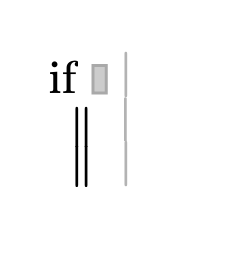
\includegraphics{new-prog-12.png}
\end{center}
В правый маркер вводится условие, в левый --- операция, которая должна быть проделана в случае, если условие выполнится (если же оно не выполняется, система просчитывает программу, пропуская данный фрагмент). Как уже говорилось, в маркер оператора может быть внесено несколько условий.

Оператор \mc{else} (Иначе) предназначен для определения того действия, которое должно быть выполнено, если условие оператора \mc{if} (Если) окажется неистинным.


\primer{Используя условные операторы, создайте блок программы для определения переменных \mc{А} и \mc{B}, которые будут принимать значения в зависимости от переменной \mc{N}. Если \mc{N>0}, то \mc{А=10}; \mc{В=20}; если \mc{N<0}, то \mc{А=5}, \mc{В=15}. Результат присвоить переменой \mc{С}.}
\begin{center}
	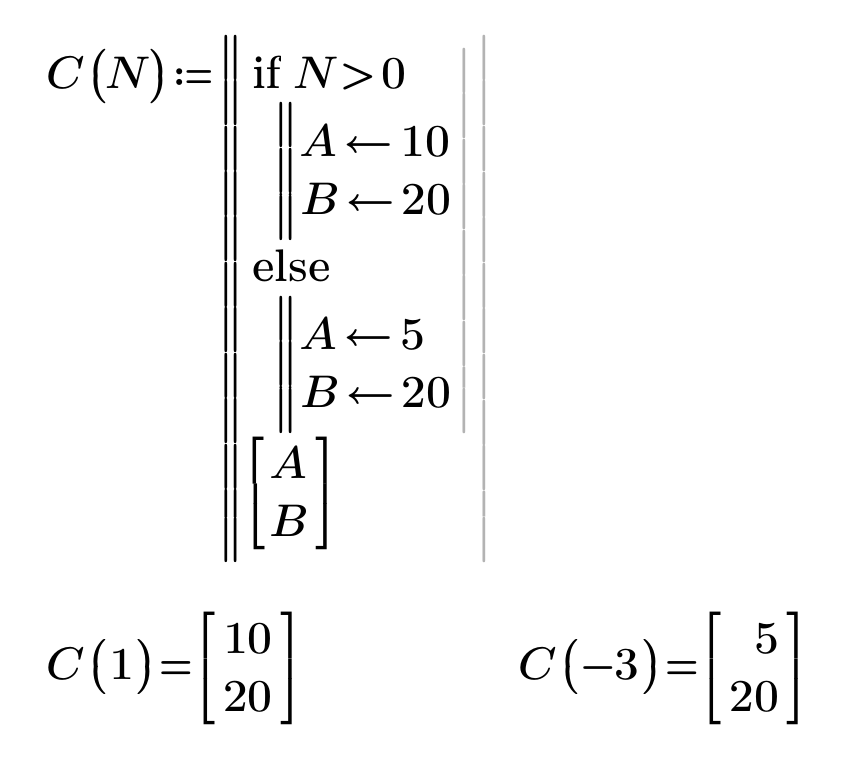
\includegraphics{new-prog-13.png}
\end{center}


Вопросы для самоконтроля:
\begin{enumerate}
	\item В какой пиктограмме содержатся операторы и элементы языка программирования Mathcad?
	\item Чем визуально отличается блок программы от остального документа?
	\item Какой оператор используется для присвоения значений переменным в программных блоках?
	\item Какие операторы цикла есть в пакете Mathcad? В чем их отличие?
	\item Какие условные операторы цикла есть в пакете Mathcad?
\end{enumerate}
